\begin{figure*}[h]
  \centering
  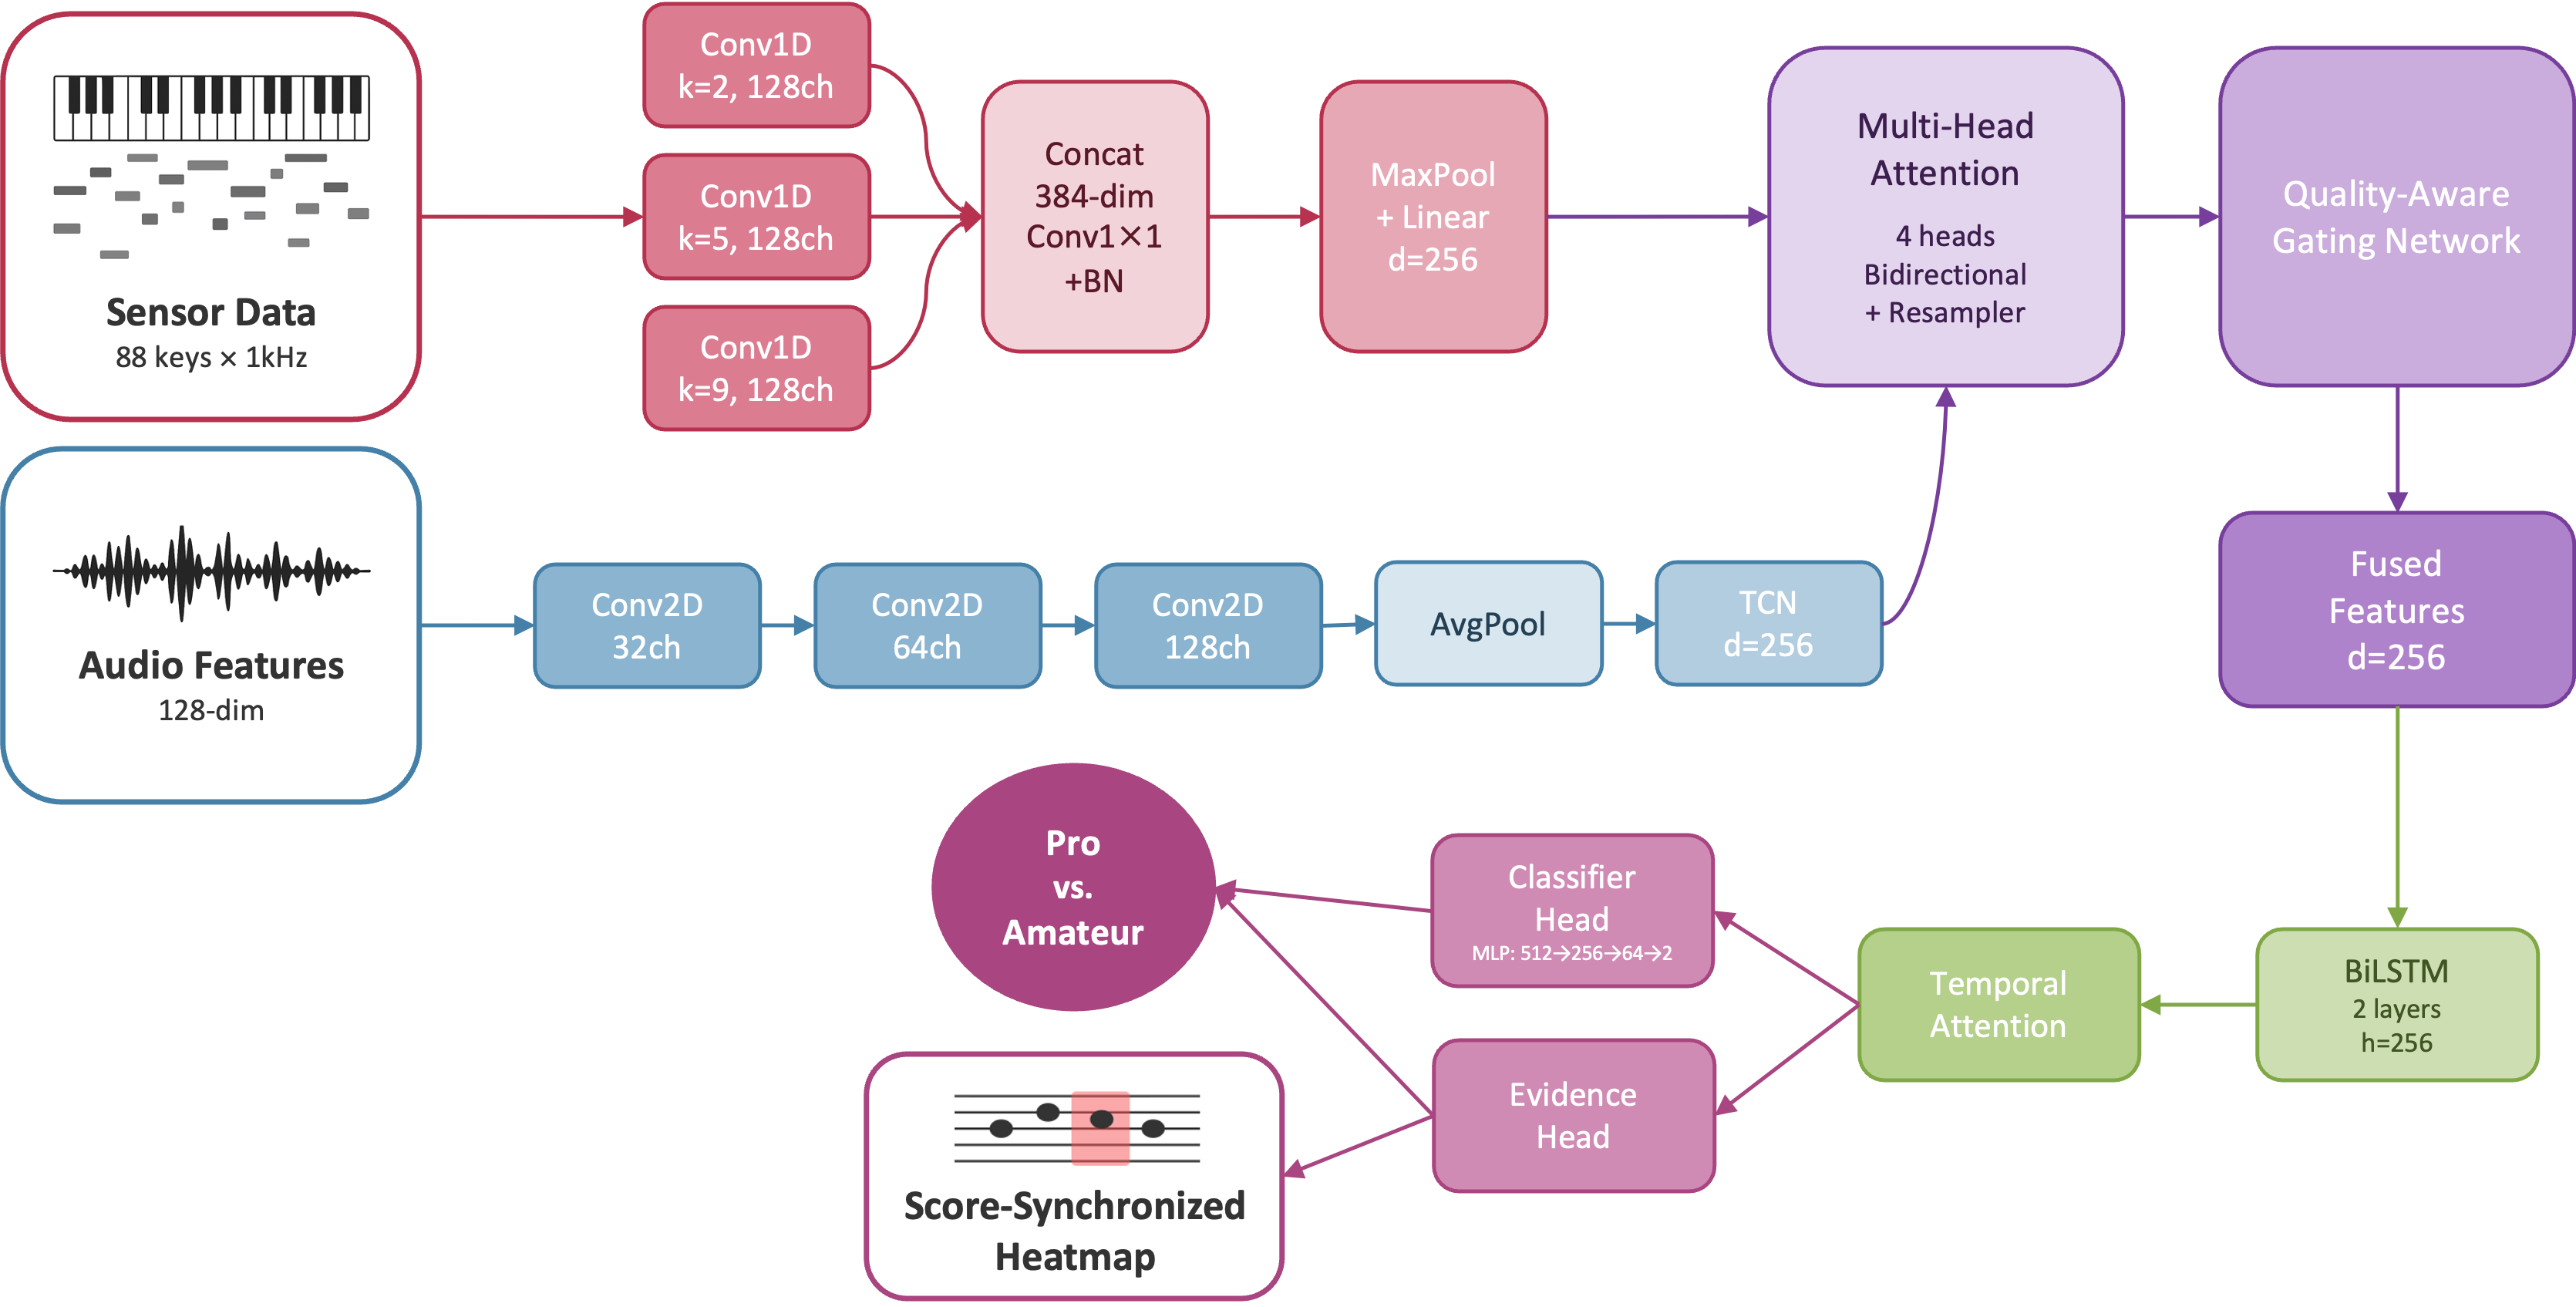
\includegraphics[width=0.8\linewidth]{figures/architecture_overview.png}
  \caption{ProfyNet architecture overview. The system processes 88-key sensor data at 1000Hz through three parallel pathways: (1) Statistical feature extraction capturing global performance metrics, (2) Dilated temporal convolutions for multi-scale pattern recognition, and (3) Local attention mechanism identifying performance-critical regions. Features are fused through learned weighting and classified via a lightweight MLP head, achieving F1=0.625 with only 288K parameters.}
  \Description{}
  \label{fig:architecture_overview}
\end{figure*}

\section{ProfyNet: Methodology and Architecture}

\subsection{Problem Formulation}

Given a piano performance with sensor data $\mathbf{S} \in \mathbb{R}^{T \times 88}$ where $T$ is the sequence length (sampled at 1000Hz) and 88 represents piano keys, our goal is to classify the performance as professional ($y=1$) or amateur ($y=0$). Additionally, we aim to produce attention weights $\mathbf{A} \in \mathbb{R}^{T}$ indicating the importance of each time step for interpretability.

The challenge lies in efficiently processing long sequences (typical performances contain 30-60 seconds = 30,000-60,000 timesteps) while capturing both local patterns (individual note articulations) and global characteristics (phrasing, dynamics).

\subsection{Statistical Feature Extraction}

Based on our empirical analysis of 859 performances, we identified six key discriminative features that capture global performance characteristics. These features complement temporal modeling by providing aggregate statistics:

\begin{equation}
\mathbf{f}_{stat} = [\sigma_v, \rho, \bar{v}, k_{sim}, n_{total}, r_v]
\end{equation}

where:
\begin{itemize}
\item $\sigma_v$: Velocity standard deviation (consistency measure)
\item $\rho$: Press density (keys/second)
\item $\bar{v}$: Average velocity (dynamic level)
\item $k_{sim}$: Simultaneous keys (chord complexity)
\item $n_{total}$: Normalized total presses (efficiency)
\item $r_v$: Velocity range (dynamic contrast)
\end{itemize}

These features are extracted efficiently in a single pass through the data:
\begin{equation}
\mathbf{f}_{stat} = \text{StatExtract}(\mathbf{S}) \in \mathbb{R}^6
\end{equation}

\subsection{Temporal Feature Extraction via Dilated Convolutions}

To capture temporal patterns at multiple scales, we employ a stack of dilated convolutional layers:

\begin{equation}
\mathbf{H}^{(l)} = \text{ReLU}(\text{BN}(\mathbf{W}^{(l)} *_d \mathbf{H}^{(l-1)} + \mathbf{b}^{(l)}))
\end{equation}

where $*_d$ denotes dilated convolution with dilation rate $d_l = 2^l$ for layer $l \in \{1,2,3\}$. This exponential dilation schedule enables receptive field growth from local (2ms) to phrasal (8ms) timescales while maintaining linear parameter growth.

The multi-scale design captures:
\begin{itemize}
\item Layer 1 ($d=1$): Note onsets and micro-timing
\item Layer 2 ($d=2$): Local articulation patterns
\item Layer 3 ($d=4$): Phrase-level structures
\end{itemize}

\subsection{Local Attention Mechanism}

Full self-attention on sequences of length $T$ requires $O(T^2)$ memory and computation, making it infeasible for our 30,000+ timestep sequences. We introduce a local attention mechanism that maintains interpretability while drastically reducing complexity:

\begin{equation}
\text{LocalAttn}(\mathbf{Q}, \mathbf{K}, \mathbf{V})_i = \text{softmax}\left(\frac{\mathbf{Q}_i \mathbf{K}_{[i-w:i+w]}^T}{\sqrt{d_k}}\right)\mathbf{V}_{[i-w:i+w]}
\end{equation}

where $w=50$ is the half-window size (100ms total window at 1000Hz). This reduces complexity from $O(T^2)$ to $O(T \cdot 2w)$, achieving 87\% reduction for typical sequences.

The window size $w=50$ was chosen based on musical considerations:
\begin{itemize}
\item Covers typical note durations (50-200ms)
\item Captures local ornamentations and articulations
\item Maintains computational efficiency
\end{itemize}

\subsection{Feature Fusion and Classification}

Temporal and statistical features are combined through learned fusion:

\begin{equation}
\mathbf{z}_{temporal} = [\text{AvgPool}(\mathbf{H}^{(L)}); \text{MaxPool}(\mathbf{H}^{(L)})]
\end{equation}

\begin{equation}
\mathbf{z}_{fused} = \text{Concat}[\alpha \cdot \mathbf{z}_{temporal}, \beta \cdot \mathbf{f}_{stat}]
\end{equation}

where $\alpha, \beta$ are learned weighting parameters initialized to 1.0.

Classification is performed via a lightweight 3-layer MLP:
\begin{equation}
\hat{y} = \text{softmax}(\text{MLP}(\mathbf{z}_{fused}))
\end{equation}

with hidden dimensions [256, 128, 2] and dropout rate 0.3 for regularization.

\subsection{Training Strategy}

\subsubsection{Loss Function}
We employ a composite loss addressing class imbalance and prediction diversity:

\begin{equation}
\mathcal{L} = \mathcal{L}_{CE} + \lambda \cdot e^{-H(\bar{p})}
\end{equation}

where $\mathcal{L}_{CE}$ is weighted cross-entropy, $H(\bar{p})$ is the entropy of average predictions across the batch, and $\lambda=0.1$ prevents mode collapse to single-class predictions.

\subsubsection{Data Balancing}
To address the 56\% professional class imbalance:
\begin{itemize}
\item Weighted random sampling: $w_c \propto 1/\sqrt{n_c}$
\item Class-weighted focal loss: $\alpha=[0.56, 0.44]$, $\gamma=2.0$
\item Augmentation: tempo variations $\pm$10\%, velocity scaling $\pm$15\%
\end{itemize}

\subsubsection{Optimization Details}
\begin{itemize}
\item Optimizer: AdamW with $lr=5 \times 10^{-4}$, $\beta=(0.9, 0.999)$
\item Weight decay: 0.01 (excluding bias and BatchNorm)
\item Gradient clipping: max norm = 1.0
\item Scheduler: ReduceLROnPlateau (patience=5, factor=0.5)
\item Early stopping: patience=10 epochs
\end{itemize}

\subsection{Implementation Efficiency}

Key optimizations for practical deployment:
\begin{itemize}
\item \textbf{Sparse operations}: Exploit sparsity in sensor data (typically 3-5 active keys)
\item \textbf{Chunked processing}: Process 3-second windows with 1-second overlap
\item \textbf{Mixed precision}: FP16 training with dynamic loss scaling
\item \textbf{Efficient attention}: Custom CUDA kernel for local attention
\end{itemize}

These optimizations enable real-time inference (< 100ms latency) on consumer GPUs.